\documentclass[oneside, fleqn, 11pt]{book}
\usepackage[a4paper, total={7.2in, 10.5in}]{geometry}
\usepackage{tikz}
\usetikzlibrary{calc}
\usepackage{setspace}
\usepackage{graphicx}
\usepackage{amsmath}
\usepackage{pgfplots}
\graphicspath{ {./images/} }
\usepackage{bookmark}
\setcounter{tocdepth}{0}

\DeclareMathOperator\dx{\mathrm{d}\mathit{x}}
\DeclareMathOperator\dy{\mathrm{d}\mathit{y}}
\DeclareMathOperator\dt{\mathrm{d}\mathit{t}}
\DeclareMathOperator\dv{\mathrm{d}\mathit{v}}
\DeclareMathOperator\dtheta{\mathrm{d}\mathit{\theta}}
\DeclareMathOperator\cis{cis}
\DeclareMathOperator\sech{sech}
\DeclareMathOperator\csch{csch}
\DeclareMathOperator\arsinh{arsinh}
\DeclareMathOperator\arcosh{arcosh}
\DeclareMathOperator\artanh{artanh}
\DeclareMathOperator\Nset{\mathbb{N}}
\DeclareMathOperator\Zset{\mathbb{Z}}
\DeclareMathOperator\Qset{\mathbb{Q}}
\DeclareMathOperator\Rset{\mathbb{R}}
\DeclareMathOperator\Iset{\mathbb{I}}
\DeclareMathOperator\Cset{\mathbb{C}}

%\usepackage[T1]{fontenc}
\usepackage{mathptmx}

\hypersetup{
	colorlinks   = true, %Colours links instead of ugly boxes
	urlcolor     = blue, %Colour for external hyperlinks
	linkcolor    = black, %Colour of internal links
	citecolor   = red %Colour of citations
}

\usepackage{hyperref}
\usepackage{blindtext}
\counterwithin*{chapter}{part}
\newcommand*{\Part}[2][\partheading]{%
  \refstepcounter{part}%
  \def\partheading{#2}%
  \part*{#2}%
  \addcontentsline{toc}{part}{#1}%
}

\newcommand{\tikzAngleOfLine}{\tikz@AngleOfLine}
\def\tikz@AngleOfLine(#1)(#2)#3{%
	\pgfmathanglebetweenpoints{%
		\pgfpointanchor{#1}{center}}{%
		\pgfpointanchor{#2}{center}}
	\pgfmathsetmacro{#3}{\pgfmathresult}%
}

\title{A Level Further Mathematics Notes - FM1}
\author{Xingzhi Lu}
\date{}

\begin{document}
\maketitle
\everymath{\displaystyle}
\tableofcontents

\chapter{Momentum and impulse}
\section{Equations}
\begin{description}
    \item[Momentum:] $p=mv$ (unit = $\text{kg m s}^{-1}$)
    \item[Impulse:] $I=\Delta mv=mv-mu=Ft$ (unit = $\text{N s}$)
\end{description}

\section{Conservation of momentum}
\begin{itemize}
    \item Momentum is always conserved in any interaction where no external forces act
    \item Elastic collision: $m_1u_1+m_2u_2=m_1v_1+m_2v_2$
    \item Sticking together: $m_1u_1+m_2u_2=(m_1+m_2)v_{1+2}$
    \item Explosion: $m_1v_1+m_2v_2=0$
\end{itemize}

\section{Momentum as a vector}
Calculate each direction independently

\chapter{Work, energy and power}
\section{Work and energy}
\begin{description}
    \item[Work done:] $w=Fd=\text{force}\times\text{distance moved in the direction of the force}=\text{change in kinetic energy}$
    \item[Kinetic energy:] $\text{K.E.}=\dfrac{1}{2}mv^2$
    \item[Potential energy:] $\text{P.E.}=mgh$
    \item[*] You must choose a \textbf{zero} level of potential energy before calculating a particle's potential energy
\end{description}



\section{Conservation of mechanical energy}
When no external forces (other than gravity) do work on a particle during its motion, the sum of the particle's \textbf{kinetic energy and (gravitational and elastic) potential energy} remains constant

\section{Work-energy principle}
The change in the total energy of a particle is equal to the work done on the particle

\section{Power}
\begin{description}
    \item[Definition:] Power is the rate of doing work
    \item[Equation:] $\text{Power}=Fv=\text{driving force produced by the engine}\times\text{velocity}$
\end{description}

\chapter{Elastic strings and springs and elastic energy}
\section{Hooke's law}
\begin{itemize}
    \item $\text{Tension produced}\propto x$ $\rightarrow$ $T=kx$, where $k$ is a constant
    \item $k$ depends on the unstretched length of the string or spring ($l$) and the \textbf{modulus of elasticity of the string or spring} ($\lambda$, unit = N)
    \item Hence $T=\dfrac{\lambda x}{l}$
    \item[*] Can also be applied if the string or spring is compressed
\end{itemize}

\section{Elastic energy}
\begin{itemize}
    \item Work done in stretching an elastic string or spring of modulus of elasticity $\lambda$ from its natural length $l$ to a length of $(l+x)$ = $\dfrac{\lambda x^2}{2l}$
    \item Elastic potential energy stored = amount of energy used to stretch the spring to a length of $(l+x)$ = $\dfrac{1}{2}kx^2$ = $\dfrac{\lambda x^2}{2l}$
    \item[*] Can also be applied when an elastic string or spring is compressed
\end{itemize}


\chapter{Elastic collisions in one dimension}
\section{Newton's law of restitution}
\begin{description}
    \item[Particles colliding:] $e=\dfrac{\text{speed of separation of particles}}{\text{speed of approach of particles}}$
    \item[Direct collision with a smooth plane:] $e=\dfrac{\text{speed of rebound}}{\text{speed of approach}}$
    \item[Range of $e$:] $0 \leq e \leq 1$
\end{description}

\section{Loss of kinetic energy}
Loss of kinetic energy due to impact = $(\dfrac{1}{2}m_1u_1^2+\dfrac{1}{2}m_2u_2^2)-(\dfrac{1}{2}m_1v_1^2+\dfrac{1}{2}m_2v_2^2)$

\section{Problems with modelling} % might need some more work here
\begin{description}
    \item[Bouncing for an infinite number of times:] the ball should stop bouncing after a finite number of bounces
    \item[Spheres modelled as particles:] air resistance is ignored
\end{description}

\chapter{Elastic collisions in two dimensions}
\section{Oblique impact with a fixed surface}
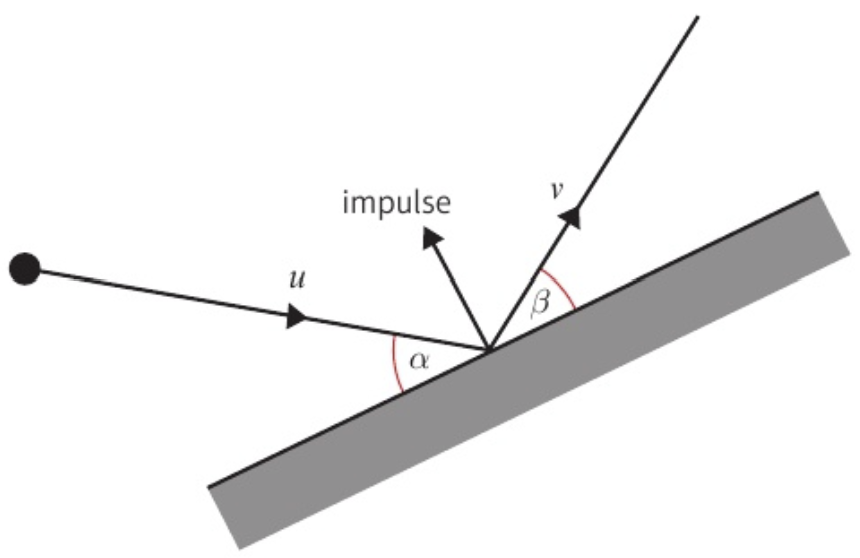
\includegraphics[width=0.3\textwidth]{obliqueimpact}
\begin{itemize}
    \item The component of the velocity of the sphere parallel to the surface is unchanged: $v\cos\beta = u\cos\alpha$
    \item The component of the velocity of the sphere perpendicular to the surface can be found with Newton's law of restitution: $v\sin\beta = eu\sin\alpha$
    \item Hence $\tan\beta = e\tan\alpha$, since $0 \leq e \leq 1$, $\beta \leq \alpha$
    \item $\text{Loss of kinetic energy}=\dfrac{1}{2}mu^2-\dfrac{1}{2}mv^2$
\end{itemize}
\section{Oblique impact of smooth spheres}
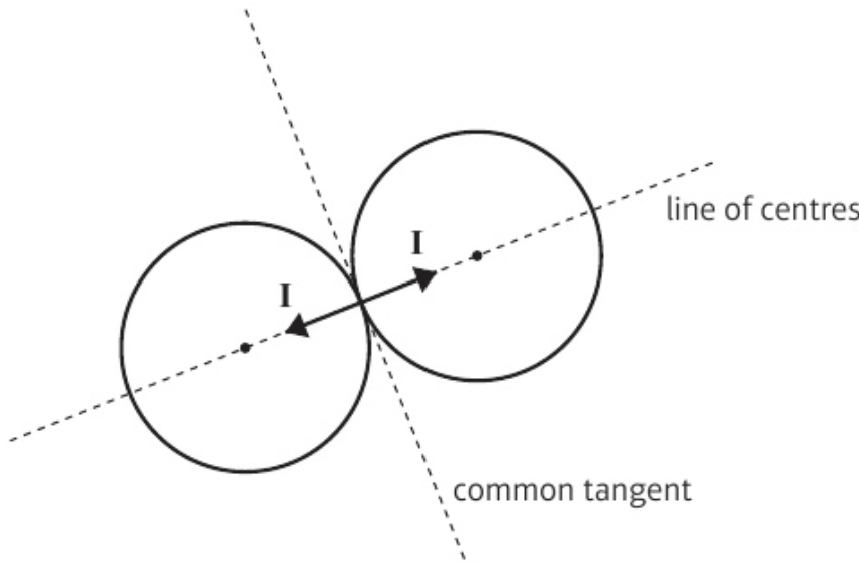
\includegraphics[width=0.3\textwidth]{oblique_2_balls}
\begin{itemize}
    \item Impulse affecting each sphere acts along the line of centres
    \item The components of the velocities of the spheres \textbf{perpendicular}  to the line of centres are unchanged in the impact
    \item The principle of conservation of momentum and Newton's law of restitution applies \textbf{parallel} to the line of centres
\end{itemize}





\end{document}